\documentclass[10pt,a4paper]{article}
\usepackage[utf8]{inputenc}
\usepackage{amsmath}
\usepackage{amsfonts}
\usepackage{amssymb}
\usepackage{graphicx}
\usepackage{listings}
\author{Maria Coto-Sarmiento}
\title{Good shit}

\begin{document}

\maketitle

\section{Introduction}




\subsection{Dataset}

We analize a dataset with amphorae from different spaces in order to understand the evolution of the amphorae. Our dataset was collected from the project \emph{Roman Amphorae: a digital recourse} within Archaeology data service at University of Southampton. \\

\begin{figure}[hbp]
	\centering
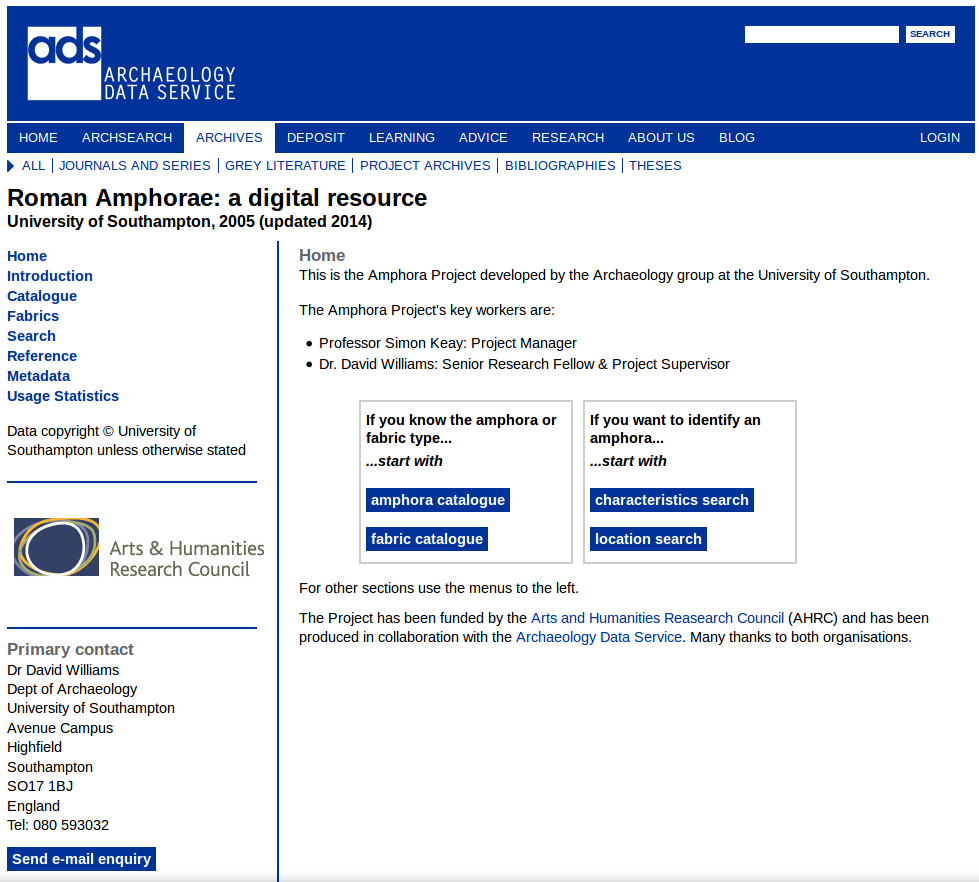
\includegraphics[scale=0.30]{picture1.png}
\label{picwebarch}
\caption{Webpage Roman Amphorae: a digital resource (Archaeology Data Service)}
\end{figure} 


This database (fig.\ref{picwebarch}) is a catalogue of aprox 375 amphorae of different types and divided from different places and chronology during the Roman Empire. We take some characteristics as the different part of the shape of amphorae and some comment to a better understanding. 

Our dataset were divided in 24 columns:

\begin{itemize}
\item[-] \textbf{id}: number of identification

\item[-] \textbf{name}: type of the amphorae 

\item[-] \textbf{rim type}: divided into triangular (the rim has two straight, angled sides, resembling two partial sides of a triangle), everted (the rim becomes gently wider towards the top), collar (the rim is noticeably thickened in the form of a collar around the neck of the amphora), beaded (a simple rounded lip), rounded (the rim is gently rounded), flaring (the rim flares out sharply, in a more pronounced manner than an everted rim), pulley wheel (this distinctive rim resembles a pulley-wheel) and beaded (a simple rounded lip. 

\item[-] \textbf{shoulder type}: divided into rounded (the shoulder is noticeably present, usually supporting the handles, but there is no ridge), carinated (the shoulder displays distinct carination - a ridge where the shoulder meets the body of the amphora) and none/smooth (there is no shoulder: the body of the amphora is uninterrupted).

\item[-] \textbf{handle profile}: divided in ear-shaped (these handles are similar to the 'curved' variety, but are more reminiscent of the shape of a human ear), bowed (the handles form a broad, curving sweep away from the body and neck of the amphora. They are generally longer than the 'curved' handles), curved (the handles gently curve from the neck to shoulder), peaked (the distinctive profile of these handles rises to a peak, often above the rim of the amphora. They are especially characteristic of the Rhodian type), ring (These handles are generally smaller than the 'curved' handles, forming a small semi-circular profile), short vertical (these handles travel upwards vertically from the shoulder, but only a short distance before turning inwards to the neck), arched(the handles form high arches, without coming to a point), long vertical(these handles generally appear on long-necked amphorae, attaching near the top of the neck progressing vertically downwards to the shoulder).

\item[-] \textbf{handle section}: divided into ovoid/elliptical (the handle appears to be ovoid or elliptical in section), ridged (the handle has one or more ridges running down it), grooved (the handle is circular, or nearly circular, in section), round (the handle is circular, or nearly circular, in section), bifid (this is a distinctive feature of the Dressel 2-4 type. The handle is formed from two rods, appearing as a figure-8 in section).

\item[-] \textbf{neck type}: divided into short/narrow (the neck is disproportionately short and/or narrow relative to the size of the amphora), cylindrical (the neck is cylinder-shaped), conical (the neck is cone-shaped - it tapers upwards), hourgrass (the neck takes the form of an hourglass, narrowing at its mid-point), none (there is no distinct neck: the body of the amphora progresses smoothly upwards to the rim), broad/wide ()

\item[-] \textbf{body type}: divided into cylindrical (the body of the amphora is cylinder-shaped, displaying little curvature), tapered (the body tapers downwards: it is wider at the top), globular (the body is wide, round and bag-shaped or globular), ovoid (the body is ovoid or elliptical in profile), piriform (the body is pear-shaped: it is wider towards the bottom of the amphora), narrow (the body is disproportionately narrow compared with the height of the amphora)

\item[-] \textbf{base type} divided into short hollow (the base is short and hollow), spike/tapered (there is a solid spike at the base of the amphora), knobbed (there is small knob at the base of the amphora), ringed (the base has a foot ring), button (there is a noticeable button-shape at the base of the amphora), flat (the base has been flattened so the amphora will stand unsupported), long hollow (the base and foot are long and hollow), pointed (the base comes to a point), rounded basal point (the base extends into a small, pronounced point - not as long as a spike)

\item[-] \textbf{capacity}: capacity of the amphorae

\item[-] \textbf{height min}: minimum height

\item[-] \textbf{height max}: maximum height

\item[-] \textbf{width min}: minimum width

\item[-] \textbf{rim diameter min}: minimum rim diameter

\item[-] \textbf{rim diameter max}: maximum rim diameter

\item[-] \textbf{manufacture}: workshops where amphorae come from

\end{itemize}


\section{Objetives}



\section{Mysql}

We use mysql and myphpadmin program with Linux to perform our data (fig.\ref{myphp})

\begin{figure}[hdp]
	\centering
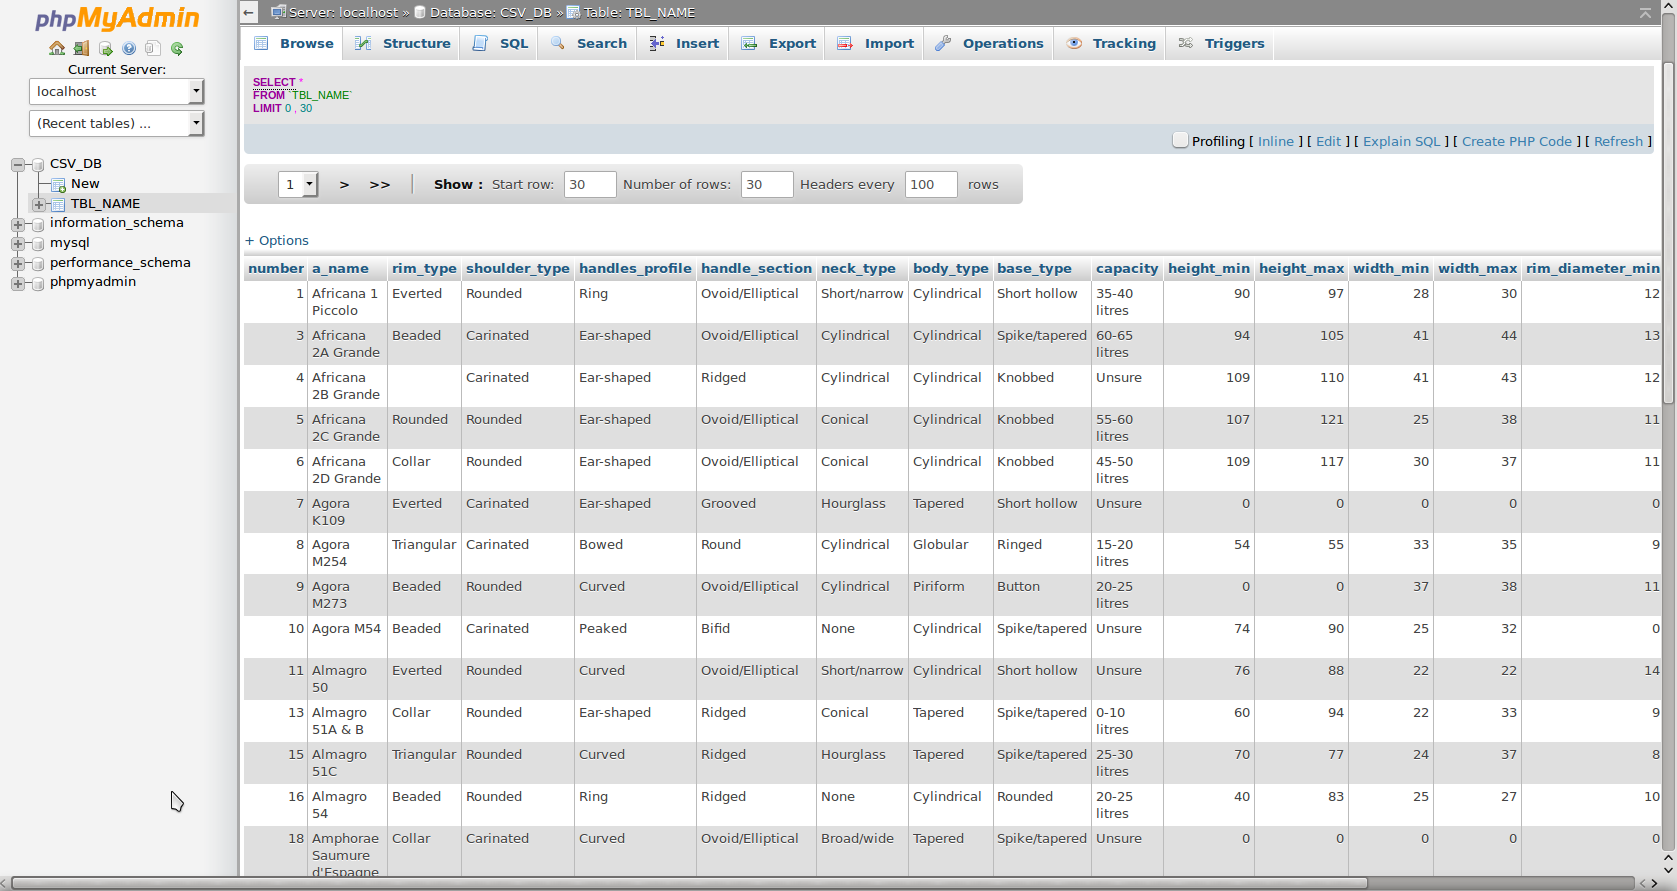
\includegraphics[scale=0.30]{picture2.png}
\label{myphp}
\caption{phpmyadmin program with the database}
\end{figure} 

\section{Mysql exercises}

\subsection{Exercise 1}

We want to know how many rim shade are everted. For that, we used the following code

\begin{verbatim}
SELECT *
FROM `TBL_NAME`
WHERE `rim_type` = "everted"
LIMIT 0 , 30
\end{verbatim}


We select all from our file but specifically we want to select from the column rim type the types which are everted. We also specify a limit by 30 (Fig. \ref{query1})

\begin{figure}[hdp]
\centering
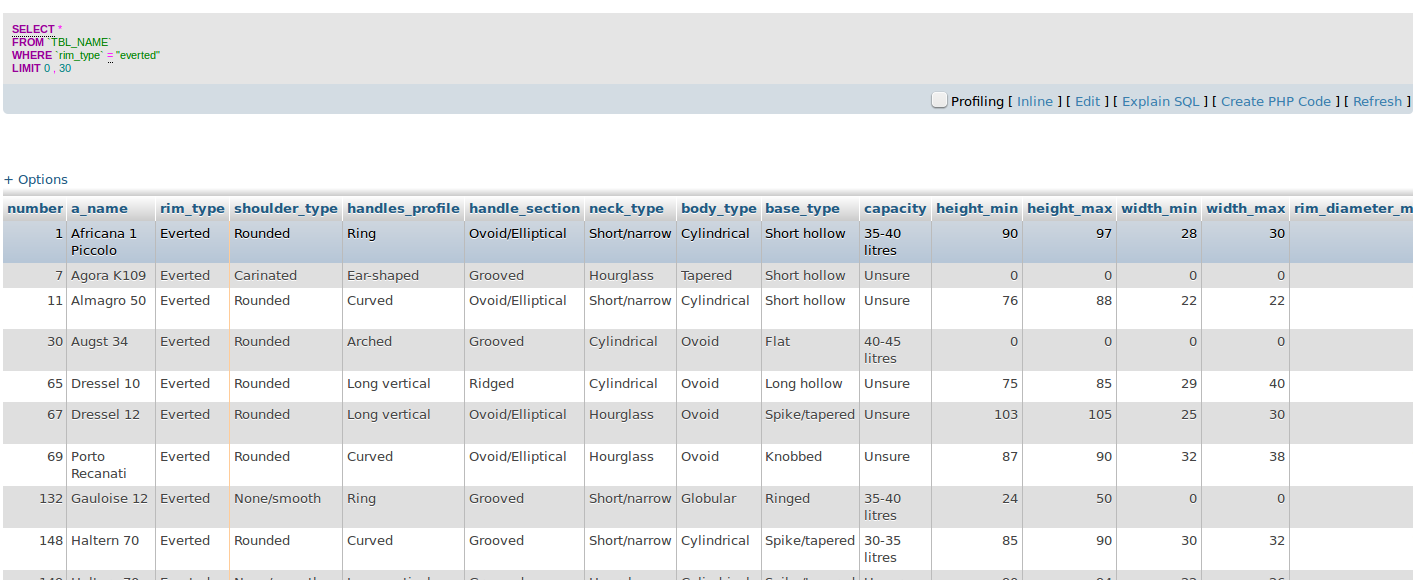
\includegraphics[scale=0.30]{output_query1.png}
\label{query1}
\caption{query selecting "everted"}
\end{figure} 


\subsection{Exercise 2}

We want to know how many amphorae have a cylindrical body type. We use the following code

\begin{verbatim}
SELECT `a_name`
FROM `TBL_NAME`
WHERE `body_type` = "cylindrical"
\end{verbatim}

We select the column $a\_name$ from the general table. Specifically, we select from the body type column which amphorae are cylindrical (Fig \ref{query2}). 

\begin{figure}[hdp]
\centering
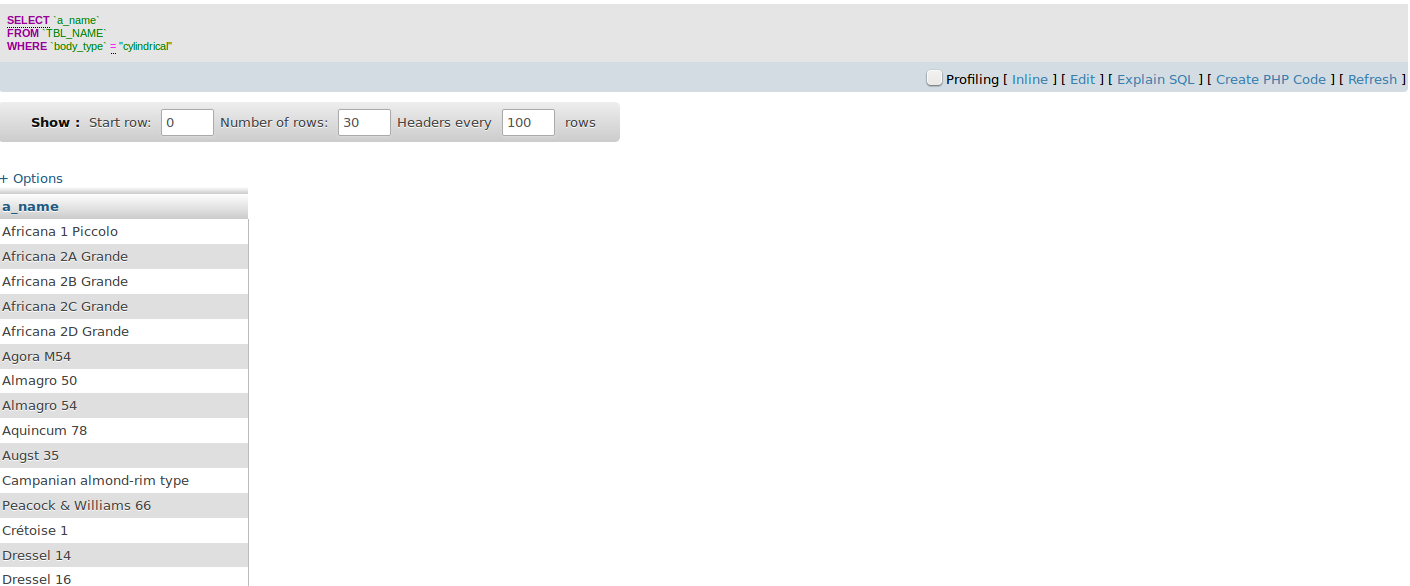
\includegraphics[scale=0.30]{query2.png}
\label{query2}
\caption{query selecting cylindrical column}
\end{figure} 


\subsection{Exercise 3}

We want to know which amphorae has the maximum diameter 

\begin{verbatim}
SELECT `a_name` , `rim_diameter_max`
FROM `TBL_NAME`
ORDER BY `rim_diameter_max` DESC
LIMIT 100 
\end{verbatim}

We select the columns and ORDER BY in order to know which diameter is bigger. We can choose betweeen ASC (ascendient order) and DESC (descendient order) (Fig \ref{query3})

\begin{figure}[hdp]
\centering
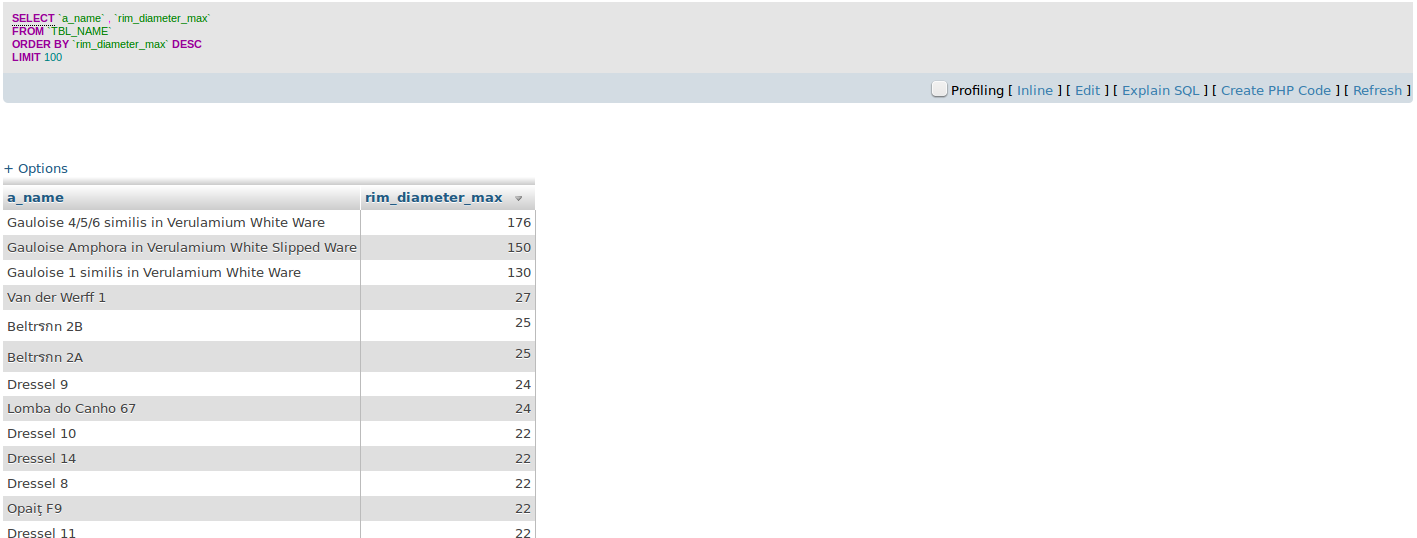
\includegraphics[scale=0.30]{query3.png}
\label{query3}
\caption{query selecting two column order by maximum diameter}
\end{figure} 

\subsection{Exercise 4}

We want to know which amphorae have cylindrical body type and carinated shoulder type with a limit of 30. We also want to order by alphabetical name of amphorae. 

\begin{verbatim}
SELECT `a_name` , `shoulder_type` , `body_type`
FROM `TBL_NAME`
WHERE `shoulder_type` = "carinated"
AND `body_type` = "cylindrical"
ORDER BY `a_name`
LIMIT 0 , 30
\end{verbatim}

We select the three columns from the original table and we specifically seelct body type and shoulder type order by names of amphorae (Fig \ref{query4})

\begin{figure}[hdp]
\centering
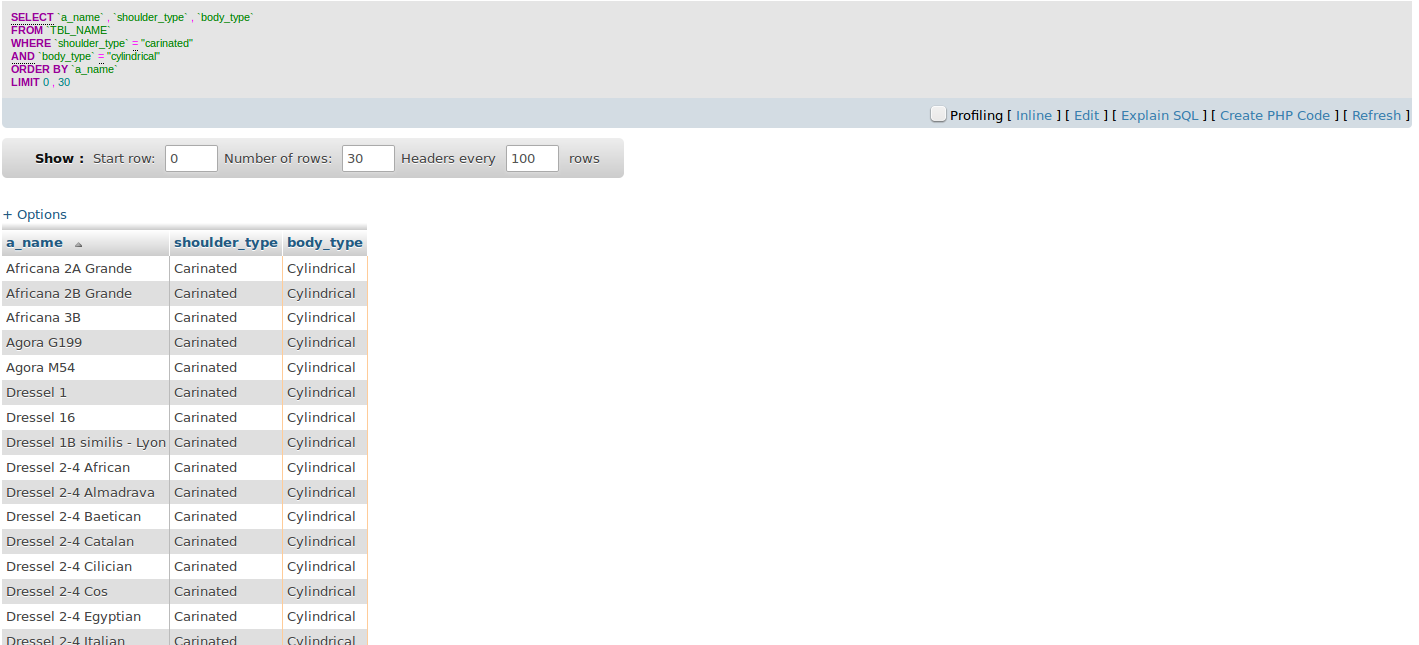
\includegraphics[scale=0.30]{query4.png}
\label{query4}
\caption{query selecting shoulder type and body type}
\end{figure} 


\subsection{Querying the data}

For our database, we want to select the Dressel types and its maximum and minimum diameter. We want to analyze the differences betweeen diameter and whether are related with the workshops. 

\begin{verbatim}
SELECT `a_name` , `rim_diameter_min` , `rim_diameter_max` , `manufacture`
FROM `TBL_NAME`
WHERE `a_name` LIKE $"%Dressel%"$
ORDER BY `a_name` ASC
LIMIT 0 , 100
\end{verbatim}

To do that, we select names of amphorae, maximum and minimum diameter and manufacture from the general table. We only want to select Dressel types so we use HACERLO to select all the Dressel on the database. The database will be ordered by names with the command order by and ascendant. The limit must be until 100 to select all the amphorae as possible (Fig \ref{query5})

\begin{figure}[hdp]
\centering
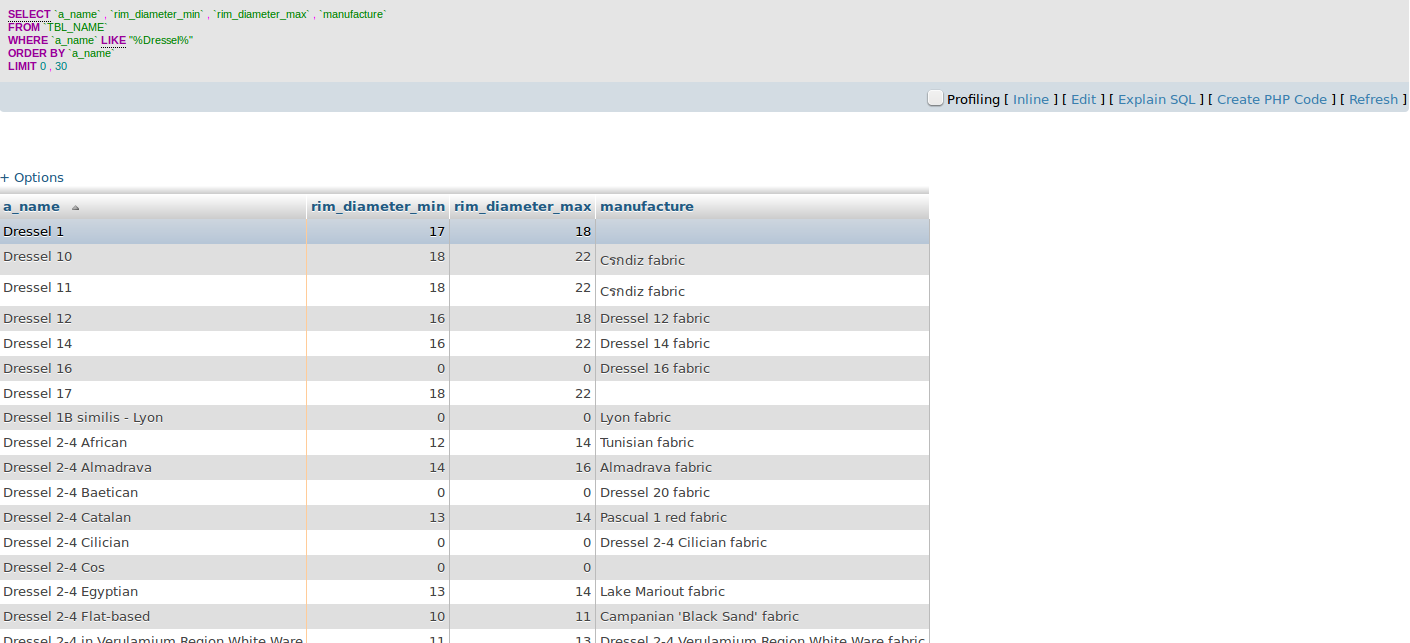
\includegraphics[scale=0.30]{query5.png}
\label{query5}
\caption{Database selected}
\end{figure} 

























 



\end{document}